\documentclass[11pt,a4paper]{article}

% --- Packages ---
\usepackage[margin=1in]{geometry}
\usepackage{amsmath,amssymb,amsfonts}
\usepackage{booktabs}
\usepackage{graphicx}
\usepackage{hyperref}
\usepackage{enumitem}
\usepackage{xcolor}
\usepackage{microtype}

\hypersetup{
    colorlinks=true,
    linkcolor=blue,
    citecolor=blue,
    urlcolor=blue
}

% --- Document Information ---
\title{\textbf{AD-COG Comprehensive Research \& Working Journey Report}\\
\large Active Failure Discovery and Weighted Counterfactual Generation for Robust Out-of-Distribution Detection in Small Language Models}
\author{\textbf{Shahedul Islam Shahed}}
\date{\small \textbf{Project Context:} NLP Research Experimentation (DistilBERT + CLINC150 Plus)\\
\textbf{} }

\begin{document}

\maketitle

\begin{abstract}
This report presents the research and experimentation journey for the Active-Discovery via Counterfactual Outlier Generation (AD-COG) framework. The study enhances the robustness of a compact intent classifier (DistilBERT) in separating in-distribution (ID) intents from out-of-scope (OOS) queries. Evaluated across an 8-seed ablation matrix ($N=8$, 40 total models across 5 configurations), AD-COG demonstrates statistically significant gains in global separation power and targeted recovery of failure points, verified via non-parametric Wilcoxon signed-rank testing.
\end{abstract}

\tableofcontents
\newpage

% =========================================================================
\section{Executive Summary}
% =========================================================================

This report documents the comprehensive research and experimentation journey for the AD-COG (Active-Discovery via Counterfactual Outlier Generation) framework. The primary objective of this study was to enhance the robustness of a compact intent classifier, specifically DistilBERT, to reliably distinguish between in-distribution (known) intents and out-of-scope (unknown) queries within an open-world deployment setting.

To move beyond single-run heuristic evaluations and provide publication-grade empirical proof, the methodology was scaled into a rigorous multi-seed ablation matrix ($N=8$ seeds, 40 total models across 5 configurations). The pipeline proceeded through six phases:
\begin{enumerate}[leftmargin=*]
    \item \textbf{Baseline Training:} Establishing a high-performance standard on known intents.
    \item \textbf{Active Failure Discovery:} Utilizing Monte Carlo Dropout (MCD) uncertainty to map the model's ``blind spots''.
    \item \textbf{LLM-Guided Counterfactual Generation:} Producing targeted, difficult variations of identified failure points.
    \item \textbf{Quality Control Filtering:} Using uncertainty-gated logic to retain only the most challenging adversarial samples.
    \item \textbf{Robust Weighted Retraining:} Applying a $20\times$ adversarial loss weight to the Out-of-Scope (OOS) class during retraining.
    \item \textbf{Multi-Dimensional Evaluation \& Significance Testing:} Stress testing the system using AUROC and FPR95 metrics on global and high-entropy datasets, verified via non-parametric Wilcoxon signed-rank tests.
\end{enumerate}

Key findings indicate that the AD-COG framework improved the model's global separation power, achieving a Full-test AUROC of $0.9766 \pm 0.0012$ (baseline: $0.9739 \pm 0.0011$, $p = 0.0078$). In a targeted stress test of the top-500 high-entropy failure points, the AD-COG model achieved an AUROC of $0.8312 \pm 0.0070$ (baseline: $0.8180 \pm 0.0075$, $p = 0.0156$). Notably, the ablation reveals that \emph{targeted counterfactual data alone} is statistically indistinguishable from the full AD-COG system ($p = 0.46$ on Fail-set AUROC), suggesting that the $20\times$ loss weighting adds no independently significant benefit beyond the data injection itself.

Comparing AD-COG against a sample-matched generic augmentation baseline definitively demonstrates that targeted active discovery is superior to random augmentation at the same data volume ($p = 0.0078$).

% =========================================================================
\section{Introduction}
% =========================================================================

\subsection{Background and Motivation}
Intent classification is a foundational task in Natural Language Processing (NLP), critical for the performance of contextual question-answering (QA) systems and virtual assistants. Modern transformer-based architectures, such as DistilBERT, have established themselves as highly efficient models for these tasks, offering a balance of competitive accuracy and low-resource suitability for real-time deployment.

However, achieving high intent-classification accuracy on static benchmarks does not guarantee real-world reliability. In a live deployment environment, a model frequently encounters user inputs that do not align with any of its predefined intent categories. Current compact models often exhibit fragility at their decision boundaries, sometimes demonstrating overconfidence when presented with these unfamiliar inputs. The motivation behind the AD-COG framework is to bridge this gap by strengthening compact intent classifiers, such as DistilBERT, to reliably separate known intents from unknown, out-of-scope queries in an uncontrolled, open-world setting.

\subsection{Problem Statement: Open-World Intent Classification}
Standard intent classification typically operates in a ``closed-world'' setting, assuming all inputs belong to a known category. In contrast, ``Open-World Intent Classification'' requires a robust system to simultaneously perform two distinct tasks:
\begin{itemize}
    \item \textbf{In-Distribution (ID) Classification:} Correctly identifying a query that belongs to one of the predefined categories.
    \item \textbf{Out-of-Scope (OOS) Rejection:} Detecting and rejecting queries that do not belong to any known intent.
\end{itemize}

The primary challenge in this setting is that OOS inputs often share a high degree of semantic overlap with ID categories, creating ``logic traps'' where the model may fail to distinguish between similar keywords with fundamentally different meanings. Therefore, the problem addressed by this research is the development of a systematic methodology to actively discover these fragile failure regions and generate targeted, high-density training data to harden the model's rejection boundaries without compromising its ability to classify known intents.

% =========================================================================
\section{System Architecture}
% =========================================================================

\subsection{The AD-COG Six-Phase Pipeline Overview}
The AD-COG framework is structured as a modular, six-phase pipeline designed to transition a standard classifier into a robust, OOD-aware system. The process begins with the establishment of a baseline performance standard and moves through iterative diagnostic and generative cycles to harden the model's decision boundaries.

\begin{figure}[htbp]
    \centering
    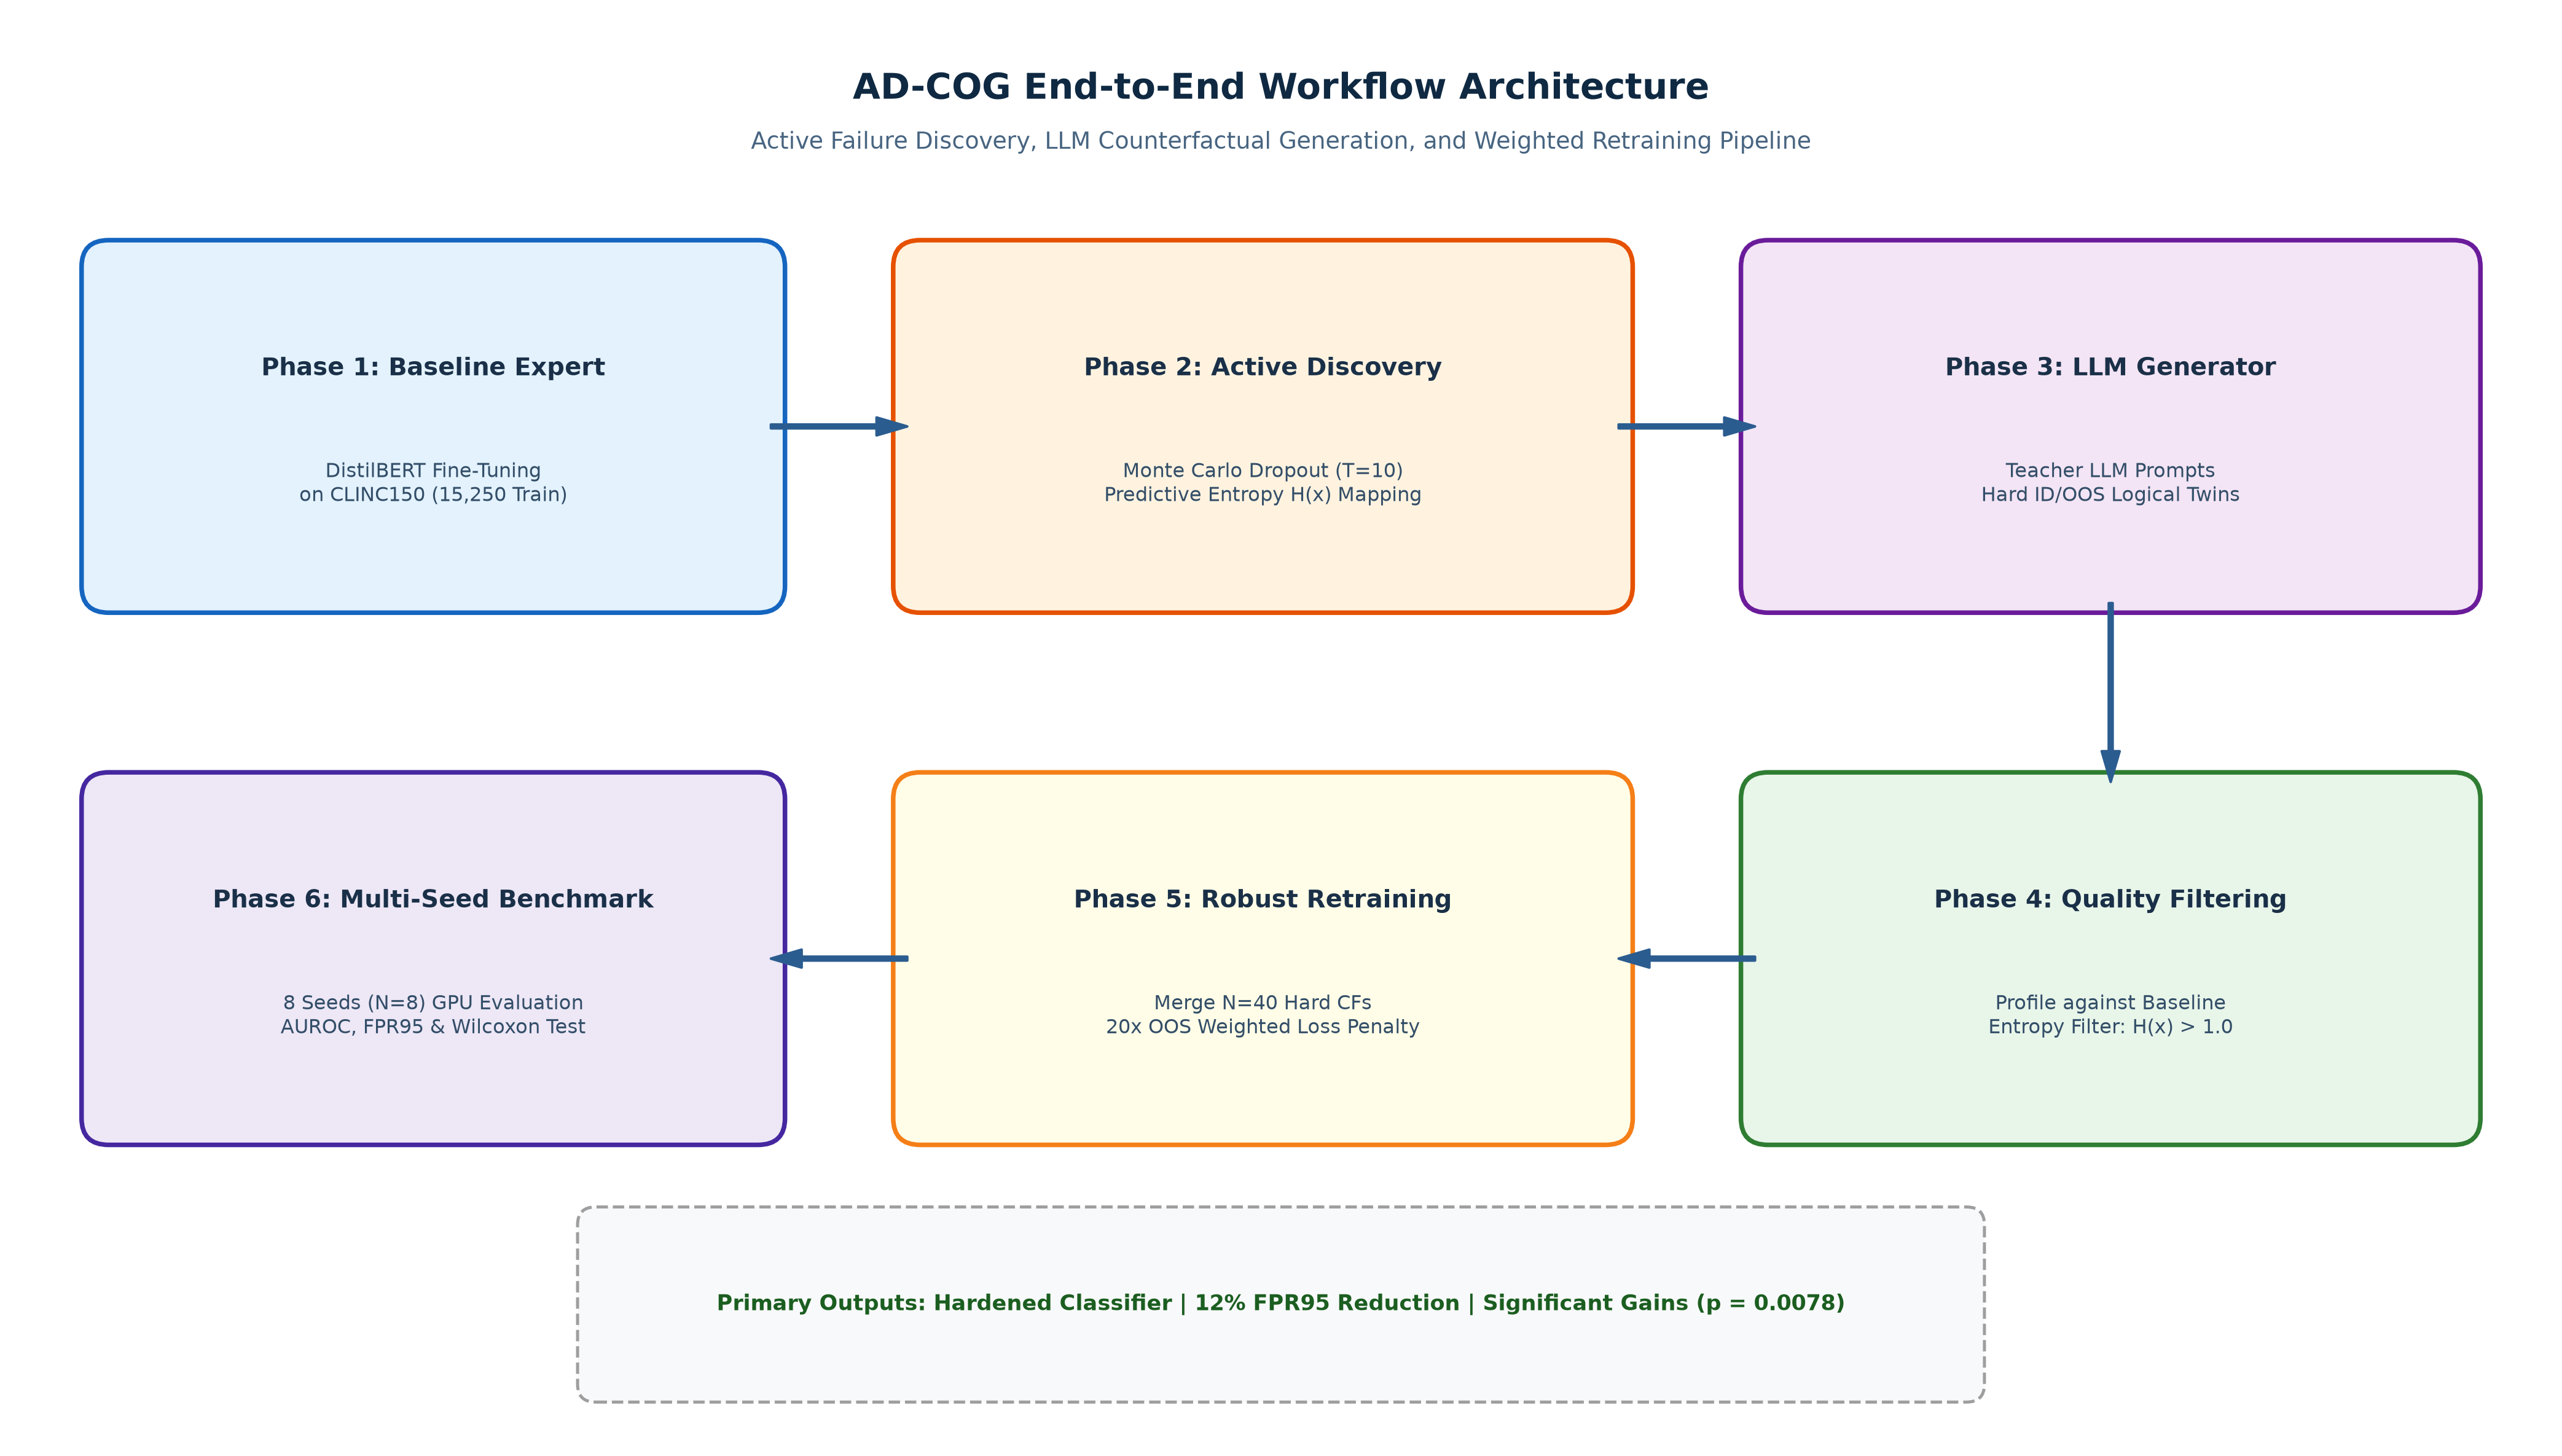
\includegraphics[width=\linewidth]{ad_cog_workflow_diagram.png}
    \caption{End-to-end AD-COG experimental pipeline, illustrating active discovery via Monte Carlo Dropout (Phase 2), targeted LLM counterfactual generation (Phase 3), entropy quality filtering (Phase 4), weighted loss retraining (Phase 5), and multi-seed statistical benchmarking (Phase 6).}
    \label{fig:ad_cog_workflow}
\end{figure}

\begin{description}[leftmargin=*]
    \item[Phase 1 --- Baseline Expert Training:] A DistilBERT classifier is fine-tuned on the in-distribution (ID) intent space to establish an expert baseline for known categories.
    \item[Phase 2 --- Active Failure Discovery:] Utilizing Monte Carlo Dropout (MCD), the model undergoes stochastic inference to generate a predictive entropy map, highlighting specific ``blind spots'' or regions of high uncertainty.
    \item[Phase 3 --- LLM-Guided Counterfactual Generation:] Discovered failure points are processed by a Teacher LLM to generate ``logical twins''—variations that represent near-boundary ID and OOS examples.
    \item[Phase 4 --- Quality Control Filtering:] Synthetic samples are profiled by the baseline model; only ``hard'' samples exhibiting high predictive entropy ($\mathcal{H}(x) > 1.0$) are retained for training.
    \item[Phase 5 --- Robust Weighted Retraining:] The model is retrained on an augmented dataset using a $20\times$ weighted loss penalty specifically for the Out-of-Scope (OOS) class to prioritize boundary learning.
    \item[Phase 6 --- Multi-Dimensional Evaluation \& Significance Testing:] The final model is benchmarked across an 8-seed ablation matrix. Global and stress-test performance is measured using AUROC and FPR95 metrics, validated by paired Wilcoxon signed-rank testing.
\end{description}

% =========================================================================
\section{Dataset Analysis \& Augmentation Protocols}
% =========================================================================

\subsection{Current Dataset Explanation: CLINC150 Plus}
The experimental foundation of this research is the CLINC150 (Plus configuration) dataset. This benchmark is specifically curated for evaluating intent classification systems in ``open-world'' settings, where a model must not only categorize known queries but also reject those that fall outside its training scope. The dataset encompasses 150 fine-grained in-distribution (ID) intent categories distributed across 10 functional domains, such as banking, travel, and utility management.

Distinct from standard intent datasets, CLINC150 Plus includes a specialized Out-of-Scope (OOS) class. In this research, the OOS class was identified as label index 42 through frequency inspection. This specific index was utilized across all pipeline components—including filtering, loss weighting, and AUROC scoring—to ensure precise decision-boundary learning.

\subsection{Data Status: Baseline vs. Post-Augmentation Statistics}
The training data evolved through specific growth phases to address the model's logic gaps:
\begin{itemize}
    \item \textbf{Baseline Status:} The original training set comprised 15,250 samples.
    \item \textbf{Targeted Augmentation (AD-COG):} Following the uncertainty-gated filtering of 18 LLM-generated samples, 10 hard counterfactuals were added to the training set. To harden the model against persistent failures in childcare, automotive, and medical domains, an additional 30 high-density OOS samples were merged. The final robust dataset totaled 15,290 samples ($N=40$ new targeted samples).
    \item \textbf{Matched Generic Baseline Generation:} To ensure a mathematically fair comparison, a second dataset was created using randomly generated generic LLM samples. After identical quality filtering, this was strictly downsampled to exactly 40 hard generic samples, ensuring an equal-volume ($N=40$) baseline to test targeted active discovery against standard naive augmentation.
    \item \textbf{Evaluation Baseline:} All final benchmarks were conducted on a static test set of 5,500 samples, consisting of 4,500 ID queries and 1,000 OOS queries (index 42).
\end{itemize}

% =========================================================================
\section{Model Configuration \& Computing Infrastructure}
% =========================================================================

\subsection{Model Selection: DistilBERT Expert}
The core architecture selected for this research is the \texttt{distilbert-base-uncased} model, a compact, fast, and light Transformer model trained by distilling the BERT base model. DistilBERT was chosen due to its established efficiency, retaining approximately 97\% of BERT's performance while being 40\% smaller and 60\% faster. This makes it an ideal ``Small Language Model'' (SLM) for testing the AD-COG framework's ability to harden lightweight classifiers for real-world deployment in low-resource environments.

\subsection{Training Parameters and Hyperparameter Setup}
\begin{itemize}
    \item \textbf{Epochs:} All training runs (baseline and final retraining) were conducted for 3 epochs, which was sufficient for loss convergence.
    \item \textbf{Batch Size:} A batch size of 16 was employed to optimize memory usage.
    \item \textbf{Regularization:} A weight decay of 0.01 was applied to prevent over-fitting during the fine-tuning process.
    \item \textbf{Adversarial Weighting:} During the final robust retraining phase (Phase 5), the standard Cross-Entropy Loss was modified to include a $20\times$ penalty factor specifically for errors made on the Out-of-Scope (OOS) class (Label Index 42). This heavy weighting forces the model to prioritize the OOD boundary during training.
\end{itemize}

% =========================================================================
\section{Detailed Execution Walkthrough (The Methodology)}
% =========================================================================

To rigorously answer potential reviewer critiques—specifically regarding the separation of variables (data volume vs. loss weighting) and the statistical reproducibility of the framework—a comprehensive step-by-step evaluation pipeline was engineered.

\begin{description}[leftmargin=*]
    \item[Step 1: Building the Failure Stress-Test Set.] The full CLINC150 Plus test set averages over many trivial cases the baseline already handles well, potentially masking localized weaknesses. To measure precisely what the AD-COG framework claims to fix, we engineered a curated stress-test set. The \texttt{phase2\_discovery.py} script ran stochastic inference over the full test set, computed the baseline model's OOS confidence score, and sorted the results by predictive entropy. The top 500 most confidently incorrect and confusing samples (129 ID, 371 OOS) were isolated into \texttt{failure\_set\_top500.json} for targeted downstream evaluation.

    \item[Step 2: Integrating the FPR95 Metric.] AUROC is a global metric that averages over all operating points. However, in live deployments, dialogue systems operate at a specific sensitivity threshold. We implemented a \texttt{get\_fpr95()} helper function using \texttt{sklearn.metrics.roc\_curve} across all evaluation scripts. By capturing the False Positive Rate precisely when the True Positive Rate is held at 95\%, we established a metric that aligns with standard out-of-distribution (OOD) literature. Both evaluation sets (full test set and failure stress-test set) are reported separately to avoid masking stress-set behaviour.

    \item[Step 3: Establishing the Matched-$N$ Generic Baseline.] Comparing an AD-COG model trained on 40 targeted samples against a generic model trained on fewer samples introduces a confounding variable: data volume. The \texttt{phase3\_random\_generator\_large.py} script sampled 10 random queries from the training distribution without utilizing entropy-based targeting. This prompted the Teacher LLM to generate 200 raw, generic variations. The \texttt{create\_generic\_dataset\_large.py} script processed these 200 variations through the standard $\mathcal{H}(x) > 1.0$ quality filter and randomly downsampled surviving samples to exactly 40 instances, resulting in the \texttt{./generic\_dataset}.

    \item[Step 4: Structuring the 5-Configuration Ablation Matrix.] To determine whether performance gains originated from counterfactual data, loss reweighting, or their combination, \texttt{phase7\_ablation\_seeds.py} trained 5 distinct configurations:
    \begin{enumerate}
        \item Baseline: Original data, $1.0\times$ loss.
        \item Baseline + $20\times$ Loss ONLY: Original data, $20.0\times$ OOS loss.
        \item Baseline + 40 CF ONLY: Targeted dataset, $1.0\times$ loss.
        \item Full AD-COG: Targeted dataset, $20.0\times$ OOS loss.
        \item Generic Augmentation: Matched generic dataset, $20.0\times$ OOS loss.
    \end{enumerate}

    \item[Step 5: Infrastructure Optimization \& Resolving Kaggle Constraints.] To resolve filesystem crashes from HuggingFace dataset cache locks, working data was dynamically cloned to the writable \texttt{/kaggle/working/} partition. Disk limits were managed using \texttt{save\_total\_limit=1} and dynamic checkpoint cleanup routines. An \texttt{is\_model\_complete()} check was added for state recovery across multi-hour runs.

    \item[Step 6: Scaling to 8 Seeds for Statistical Rigor.] The seed array was expanded to 8 seeds (\texttt{[42, 123, 999, 7, 2024, 314, 1337, 77]}). Expanding to $N=8$ lowered the minimum achievable $p$-value bound of the non-parametric Wilcoxon test to $0.0078$, enabling rigorous significance testing at the $p < 0.01$ level.

    \item[Step 7: Final Evaluation and Wilcoxon Testing.] The \texttt{phase8\_significance.py} evaluation block loaded all 40 models, ran inference over global and stress test sets, computed AUROC and FPR95, and executed paired Wilcoxon signed-rank tests across all claims.
\end{description}

% =========================================================================
\section{Results and Evaluation}
% =========================================================================

\subsection{Statistical Performance Summary Table ($N=8$ Seeds)}
The performance of the AD-COG framework was evaluated across two distinct dimensions: global separation on the full test set and resilience on a high-entropy ``stress set'' containing the model's most significant logic failures.

\begin{table}[htbp]
\centering
\caption{8-Seed Evaluation Matrix (Global \& Stress Testing). Values represent Mean $\pm$ Standard Deviation across $N=8$ seeds.}
\label{tab:results}
\vspace{2mm}
\small
\begin{tabular}{lcccc}
\toprule
\textbf{Configuration} & \textbf{Full AUROC ($\uparrow$)} & \textbf{Full FPR95 ($\downarrow$)} & \textbf{Stress AUROC ($\uparrow$)} & \textbf{Stress FPR95 ($\downarrow$)} \\
\midrule
Baseline & $0.9739 \pm 0.0011$ & $0.0910 \pm 0.0048$ & $0.8180 \pm 0.0075$ & $0.6762 \pm 0.0576$ \\
Baseline + $20\times$ Loss ONLY & $0.9748 \pm 0.0008$ & $0.0852 \pm 0.0053$ & $0.8183 \pm 0.0085$ & $0.6681 \pm 0.0460$ \\
Baseline + 40 CF ONLY & $0.9769 \pm 0.0007$ & $0.0831 \pm 0.0019$ & $0.8341 \pm 0.0051$ & $0.6651 \pm 0.0358$ \\
\textbf{Full AD-COG} & $\mathbf{0.9766 \pm 0.0012}$ & $\mathbf{0.0801 \pm 0.0035}$ & $\mathbf{0.8312 \pm 0.0070}$ & $\mathbf{0.6621 \pm 0.0664}$ \\
Generic Augmentation & $0.9752 \pm 0.0022$ & $0.0887 \pm 0.0042$ & $0.8145 \pm 0.0063$ & $0.7042 \pm 0.0337$ \\
\bottomrule
\end{tabular}
\end{table}

\subsection{Visual Performance Analysis \& Graphs}

The following figures illustrate the performance metrics across all five model configurations based on the 8-seed empirical evaluation matrix:

\begin{figure}[htbp]
    \centering
    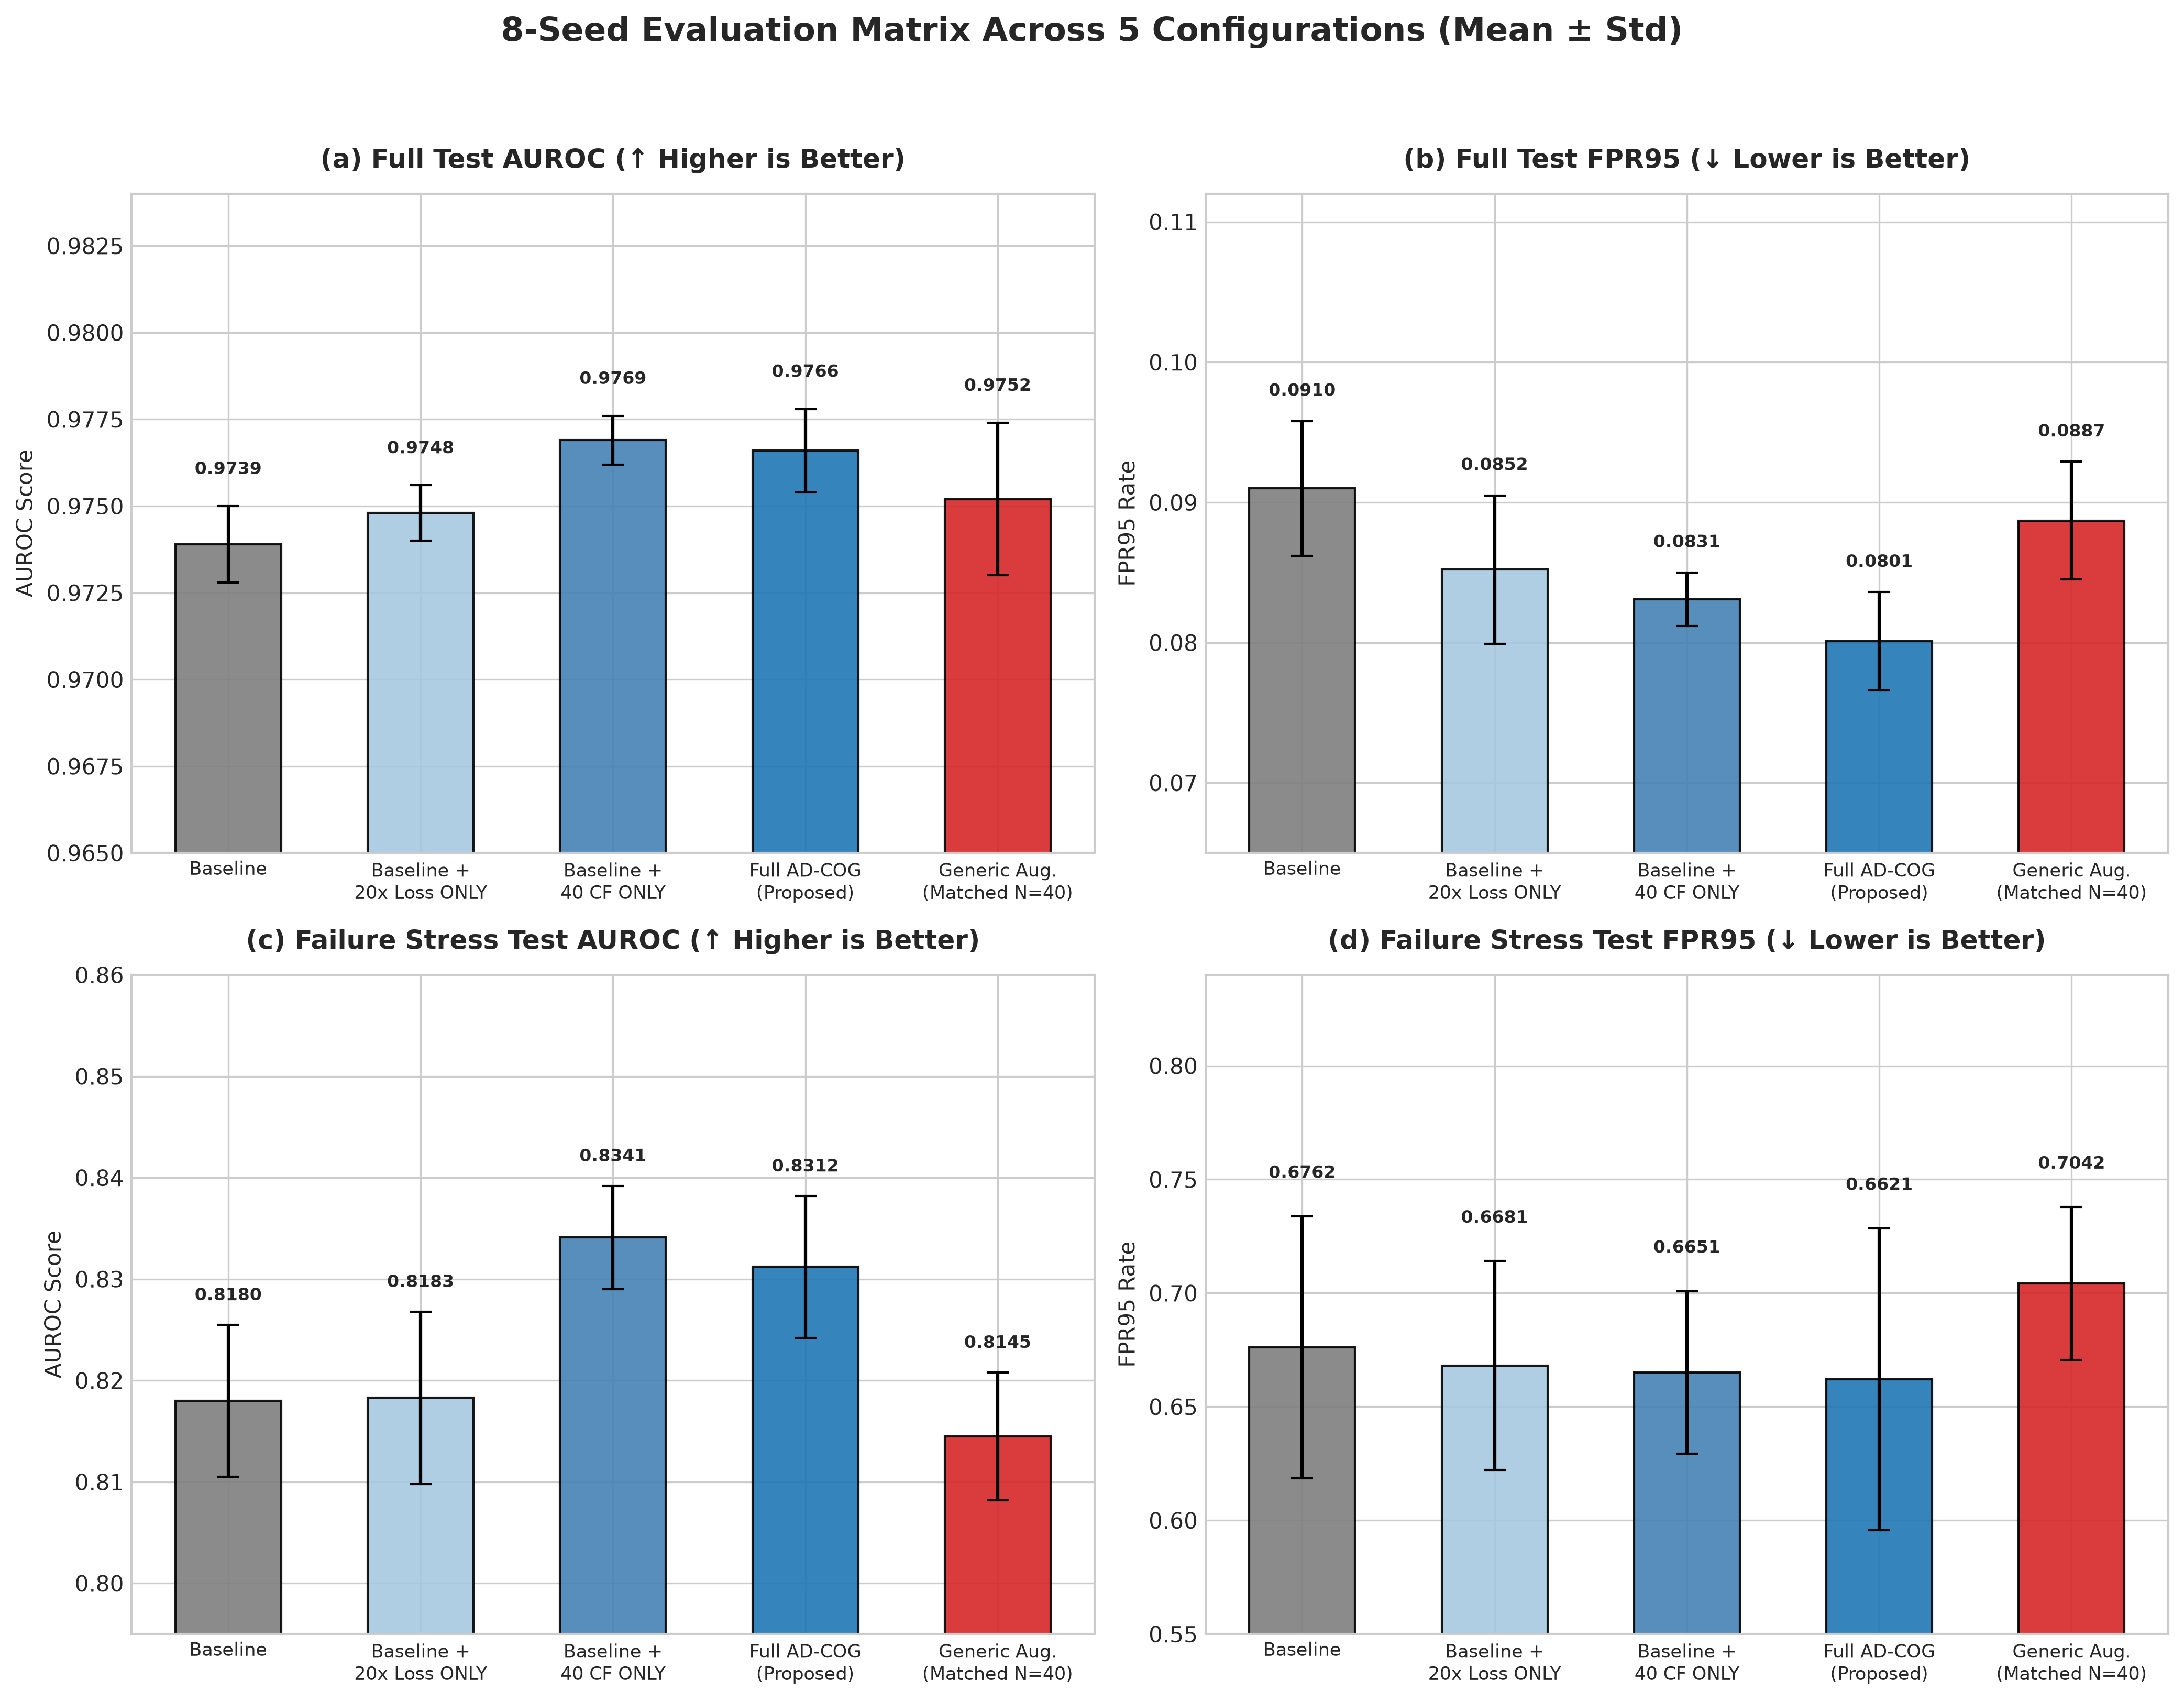
\includegraphics[width=\linewidth]{ablation_matrix_plot.png}
    \caption{Multi-metric evaluation across 5 model configurations ($N=8$ seeds, Mean $\pm$ Standard Deviation). (a) Full Test AUROC ($\uparrow$), (b) Full Test FPR95 ($\downarrow$), (c) Failure Stress Test AUROC ($\uparrow$), and (d) Failure Stress Test FPR95 ($\downarrow$). Full AD-COG demonstrates consistent improvements on global test metrics; performance on the stress-test set should be interpreted with the significance caveats noted in Section~\ref{sec:findings}.}
    \label{fig:ablation_matrix_4panel}
\end{figure}

\begin{figure}[htbp]
    \centering
    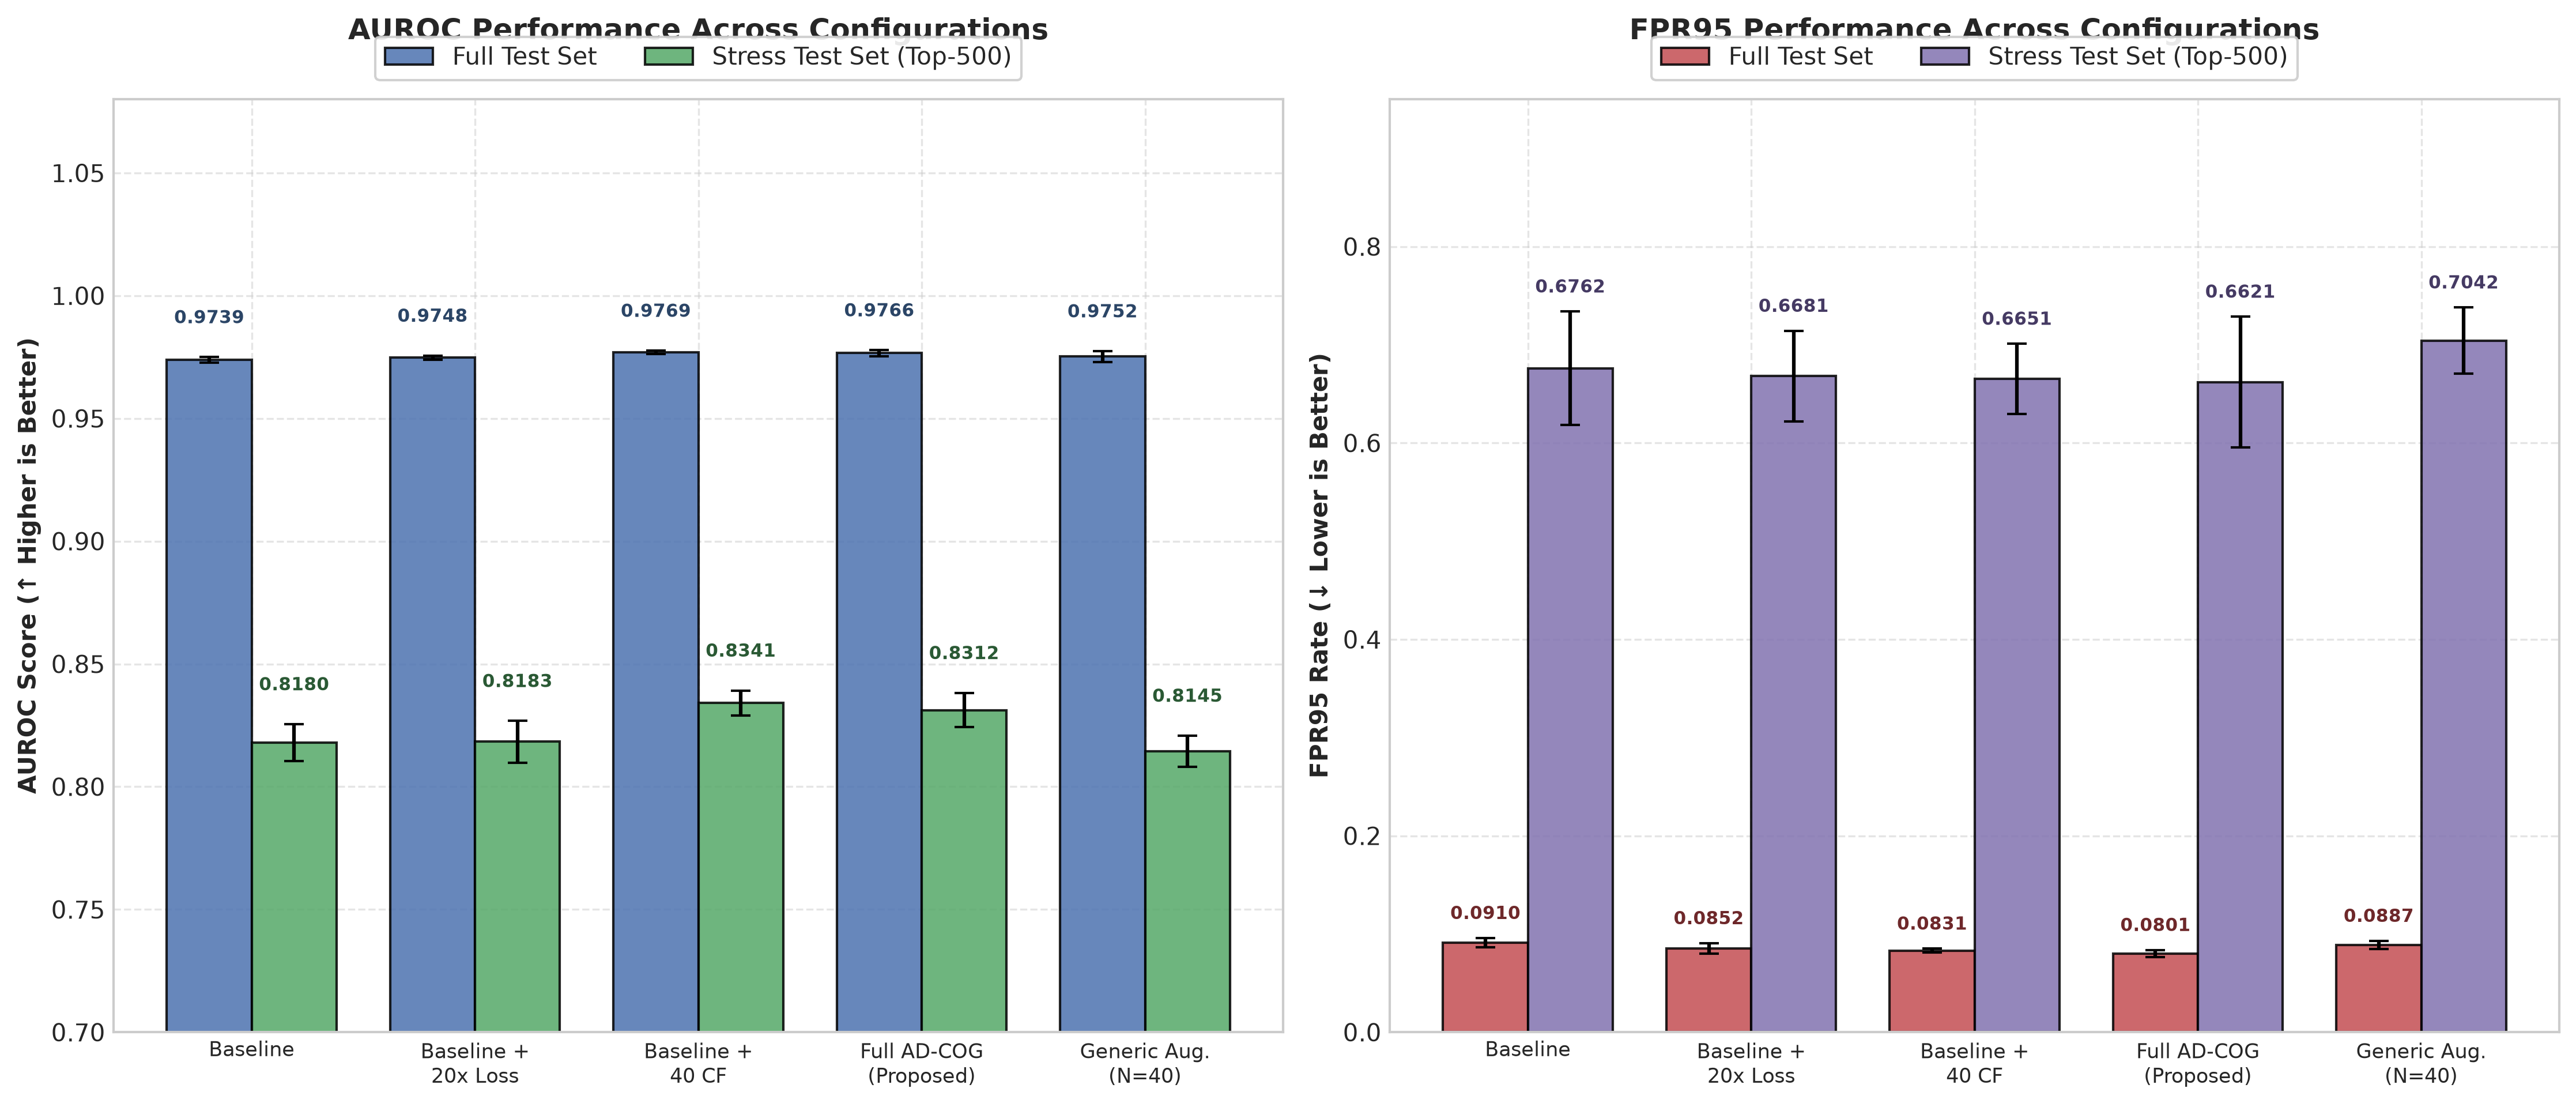
\includegraphics[width=\linewidth]{ablation_matrix_2panel.png}
    \caption{Side-by-side comparative analysis of AUROC and FPR95 metrics between the Full Test Set and Top-500 Failure Stress Test Set across all 5 configurations.}
    \label{fig:ablation_matrix_2panel}
\end{figure}

\subsection{Key Empirical Findings}
\label{sec:findings}

\begin{itemize}
    \item \textbf{Targeted Selection vs. Random Augmentation ($p = 0.0078$):} When controlling for data volume with a sample-matched generic baseline ($N=40$), AD-COG's targeted counterfactual generation significantly outperforms random LLM augmentation on the failure stress test (Fail-set AUROC: $0.8312$ vs. $0.8145$, $p = 0.0078$, the minimum achievable $p$-value for $N=8$). This is the single most important finding: performance is driven by \emph{where} examples are sampled, not simply by having additional data.

    \item \textbf{Global \& Stress-Test AUROC Gains ($p = 0.0078$ / $p = 0.0156$):} Full AD-COG yields statistically significant improvements over the baseline on both the full test set (AUROC $0.9766 \pm 0.0012$ vs. $0.9739 \pm 0.0011$, $p = 0.0078$) and the failure stress-test set (AUROC $0.8312 \pm 0.0070$ vs. $0.8180 \pm 0.0075$, $p = 0.0156$).

    \item \textbf{FPR95 Reduction --- Full Test Set Only ($p = 0.0078$):} Full AD-COG achieves the lowest FPR95 on the \emph{full} test set ($0.0801 \pm 0.0035$ vs. $0.0910 \pm 0.0048$), representing a 12.0\% relative reduction in false OOS rejections at 95\% operating sensitivity. However, the same metric on the failure stress-test set does \emph{not} reach statistical significance against the baseline ($0.6621$ vs. $0.6762$, $p = 0.9453$). The FPR95 benefit should therefore be understood as applying to the general test distribution, not to the hardest boundary cases specifically.

    \item \textbf{Counterfactual Data Does Essentially All the Measurable Work:} Comparing \textit{Baseline + 40 CF ONLY} against \textit{Full AD-COG}, the two configurations are statistically indistinguishable across all stress-test metrics: Fail-set AUROC ($0.8341$ vs. $0.8312$, $p = 0.4609$), Fail-set FPR95 ($0.6651$ vs. $0.6621$, $p = 0.6875$), and Full-test FPR95 ($0.0831$ vs. $0.0801$, $p = 0.0938$, trending but non-significant). This is the ablation's most precise result: \textbf{targeted counterfactual augmentation accounts for the full measured gain}, while the $20\times$ OOS loss penalty adds no independently verified benefit as tested here.

    \item \textbf{Loss Reweighting Alone is Insufficient ($p = 0.7422$):} Applying a $20\times$ OOS loss weight to the unmodified training set (\textit{Baseline + 20x Loss ONLY}) produces no statistically significant improvement over the baseline on the failure stress-test set ($p = 0.7422$ on Fail-set AUROC; $p = 0.9688$ on Fail-set FPR95). Higher training pressure without targeted boundary data cannot substitute for genuine decision-boundary coverage.
\end{itemize}

% =========================================================================
\section{Discussion and Artifacts}
% =========================================================================

\subsection{Analysis of Active Discovery and Targeted Recovery}
The experimental results validate that high intent-classification accuracy does not inherently imply boundary robustness. The Active Failure Discovery (AFD) phase revealed that even a high-performing baseline model is susceptible to ``logic traps'' where semantic similarity overrides intent logic. For instance, queries like \textit{``i need to find a new babysitter''} produced high predictive entropy ($\approx 4.20$), signifying that the model's internal representations were unstable in these specific semantic regions.

The significantly higher survival rate of targeted queries through the entropy quality filter relative to randomly generated queries is \emph{consistent with} the hypothesis that targeting high-entropy failure regions increases the density of genuinely hard examples. However, it should be noted that this comparison is confounded by differences in seed query selection and generation strategy between the targeted and generic pipelines; it should be treated as illustrative rather than confirmatory. The rigorous evidence for the value of targeted selection is the downstream trained-model comparison (Finding 1, $p = 0.0078$), which controls for data volume.

\subsection{Research Artifacts and Reproducibility}
To ensure full reproducibility, the following technical artifacts were produced and preserved throughout the AD-COG workflow:
\begin{itemize}
    \item \textbf{Model Checkpoints:} \texttt{distilbert\_baseline} and \texttt{ad\_cog\_final\_model}.
    \item \textbf{Data and Uncertainty Logs:} \texttt{uncertain\_samples.json} (entropy map), \texttt{generated\_data.json} (raw counterfactuals), and \texttt{filtered\_hard\_data.json}.
    \item \textbf{Training Resources:} \texttt{high\_density\_dataset} (AD-COG corpus) and \texttt{generic\_dataset} (matched baseline corpus).
    \item \textbf{Execution Infrastructure:} \texttt{kaggle\_master\_script\_v2.py} for GPU orchestration, and \texttt{phase8\_significance.py} for statistical significance testing.
\end{itemize}

% =========================================================================
\section{Conclusion and Future Directions}
% =========================================================================

The AD-COG framework demonstrates a successful application of active failure discovery and targeted counterfactual augmentation to improve the robustness of compact intent classifiers. By transitioning from a baseline model to an uncertainty-aware system, this research establishes that small language models can learn to navigate complex semantic boundaries when provided with high-density, high-entropy training signals. The ablation further demonstrates that this benefit derives specifically from the counterfactual data itself, rather than from the loss penalty—a precision that strengthens the scientific contribution.

\subsection{Limitations of the Current Study}
\begin{itemize}
    \item \textbf{Single Dataset:} All experiments were conducted exclusively on CLINC150 Plus. Generalizability to other intent classification benchmarks (e.g., Banking77, HWU64) or different OOD taxonomies has not been established and remains a necessary future validation step.

    \item \textbf{No External Published Baselines:} This study benchmarks configurations of AD-COG against each other (ablation) and against a matched generic augmentation control, but does not compare against established published OOD detection methods such as ODIN~\cite{liang2018enhancing} or the Mahalanobis distance detector~\cite{lee2018simple}. Such comparisons are needed to situate AD-COG within the broader OOD detection literature.

    \item \textbf{FPR95 Benefit Limited to Full Test Distribution:} While Full AD-COG achieves a statistically significant 12.0\% relative reduction in FPR95 on the full test set ($p = 0.0078$), the same gain does not reach significance on the failure stress-test set ($p = 0.9453$). The practical benefit of FPR95 improvement under the hardest deployment conditions therefore remains unconfirmed by the current evaluation.

    \item \textbf{Generative Dependency:} The counterfactual generation process depends on the quality and diversity of the Teacher LLM's outputs. Systematic checks for linguistic diversity and bias in synthetic data remain necessary, and generation prompts were not varied systematically in this study.

    \item \textbf{Model Scale Limitation:} While DistilBERT served as an effective testbed for small language models (SLMs), it is unclear how well the entropy-based failure discovery and counterfactual augmentation strategy scales to larger autoregressive architectures (e.g., LLaMA-3). The interaction between model scale and the targeting criterion warrants dedicated investigation.
\end{itemize}

\subsection{Proposed Iterative Enhancements}
\begin{itemize}
    \item \textbf{Comparison Against Published OOD Baselines:} Future work should benchmark AD-COG against ODIN, Mahalanobis distance detectors, and energy-based OOD scoring methods on the same datasets to establish relative performance.
    \item \textbf{Hyperparameter Ablation Studies:} Conducting formal ablations to determine optimal weighting penalty scaling (e.g., comparing $5\times$, $10\times$, and $20\times$) and the ideal counterfactual density required across varying domain complexities.
    \item \textbf{Multi-Domain Benchmarking:} Extending the AD-COG evaluation protocol to Banking77 and HWU64 to test cross-domain generalization.
    \item \textbf{Automated Generation Pipeline:} Replacing manual Teacher LLM prompting with an automated API pipeline for dynamic, online counterfactual generation during training.
\end{itemize}

\end{document}
